
\begin{center}
\textbf{Alimentation des canons à neige}
\end{center}

%L'enneigement artificiel des stations de ski est une pratique relativement récente en Europe et en Amérique du Nord. C'est un procédé nécessaire au maintien et au développement des activités économiques d'une station. Or, la production de neige nécessite de grands volumes d'eau pompés dans les rivières, les nappes phréatiques, les barrages hydroélectriques et les retenues collinaires.

Aujourd'hui, la plupart des stations de ski construisent des retenues d'eau en altitude afin d'alimenter les canons à neige placés le long des pistes en aval. %La surface qu'il est possible de recouvrir en neige artificielle dépend du volume d'eau stockée dans la retenue.

%Il faut environ un volume de 4 000 m$^3$ d'eau pour couvrir de neige et rendre skiable une surface d'un hectare.

Pour répondre à ses besoins, une station a décidé de réaliser un bassin dont la vue de dessus a la forme ci-dessous. %et d'une profondeur telle que le volume d'eau contenu présente une hauteur $h$ maximale de 8 m.

%L'objectif est de déterminer si la quantité d'eau liquide retenue dans le bassin lorsque celui-ci est rempli permet de couvrir de neige une surface de 14 hectares.

Au niveau du sol, le tour du bassin peut être modélisé par la courbe fermée représentée sur la figure ci-dessous.

Avec l'échelle utilisée sur le graphique, 1 unité correspond à 15 m :

\medskip

\begin{center}
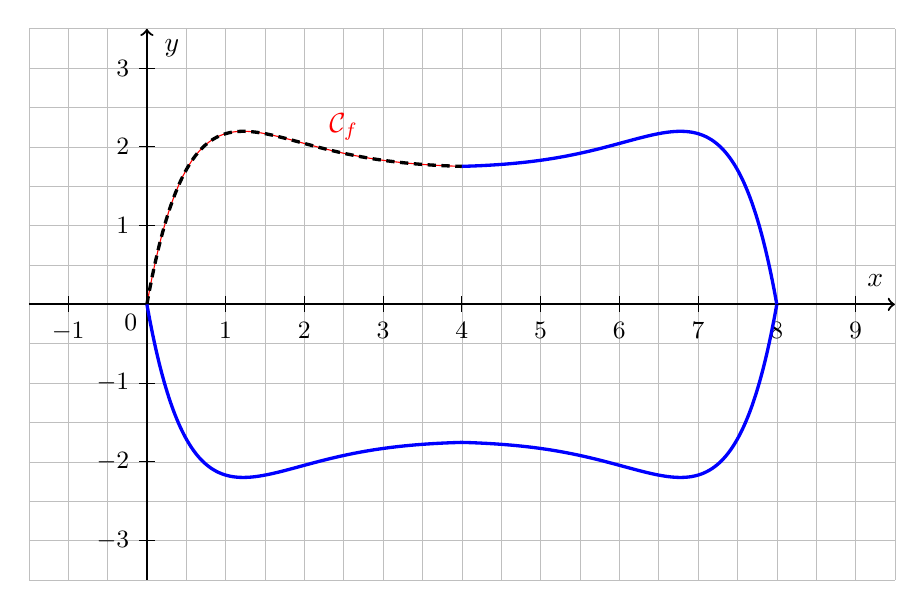
\begin{tikzpicture}
    % Configuration de la grille
    \draw[step=0.5,gray!50,very thin] (-1.5,-3.5) grid (9.5,3.5);

    % Axes
    \draw[->,thick] (-1.5,0) -- (9.5,0);
    \draw[->,thick] (0,-3.5) -- (0,3.5);

    % Labels des axes
    \node[above] at (9.25,0.1) {$x$};
    \node[right] at (0.1,3.25) {$y$};

    % Marques des axes
    \foreach \x in {-1,1,2,...,9} {
        \draw (\x,0.1) -- (\x,-0.1) node[below] {\small $\x$};
    }
    \foreach \y in {-3,-2,-1,1,2,3} {
        \draw (0.1,\y) -- (-0.1,\y) node[left] {\small $\y$};
    }
    % Marque spéciale pour 0
    \node[below left] at (0,0) {\small $0$};
    
    % Tracé de la fonction f-1(x)
    \draw[domain=0:4,samples=200,smooth,red,thin] plot (\x, {-(\x*\x - 3.8*\x + 1.8)*exp(-\x) + 1.8});
    \draw[domain=0:4,samples=200,smooth,black,very thick,densely dashed] plot (\x, {-(\x*\x - 3.8*\x + 1.8)*exp(-\x) + 1.8});
    
    % Tracé de la fonction f-2(x)
    \draw[domain=0:4,samples=200,smooth,blue,very thick] plot (\x, {(\x*\x - 3.8*\x + 1.8)*exp(-\x) - 1.8});
    
    % Tracé du symétrique de f-1(x) par rapport à x=4
    \draw[domain=4:8,samples=200,smooth,blue,very thick] plot (\x, {-( (8-\x)*(8-\x) - 3.8*(8-\x) + 1.8)*exp(-(8-\x)) + 1.8});
    
    % Tracé du symétrique de f-2(x) par rapport à x=4
    \draw[domain=4:8,samples=200,smooth,blue,very thick] plot (\x, {((8-\x)*(8-\x) - 3.8*(8-\x) + 1.8)*exp(-(8-\x)) - 1.8});
    
    % Label de f-1(x)
    \node[red] at (2.5,2.25) {$\mathcal{C}_f$};
\end{tikzpicture}
\end{center}
\vspace{-2em}
\begin{center}
    \textit{Tour du bassin au niveau du sol.}
\end{center}

%\textbf{Calcul de la surface du bassin au niveau du sol.}

Le tour du bassin au niveau du sol présente deux axes de symétrie : l'axe des abscisses et la droite d'équation $x = 4$. Il est obtenu par symétrie de la courbe $\mathcal{C}_f$ tracée en pointillé sur la figure.

La courbe $\mathcal{C}_f$ est représentative de la fonction $f$ définie pour tout réel sur l'intervalle $[0\,;\,4]$ par :
\[f(x) = -(x^2 - 3,8x + 1,8)\e^{-x} + 1,8.\]
Sur l'intervalle $[0\,;\,4]$, on admet que la fonction $f$ est positive.

\begin{enumerate}
\item Montrer que la fonction $f$ admet comme primitive sur $\mathbb{R}$ la fonction $F$ définie pour tout réel $x$ par :
\[F(x) = (x^2 - 1,8x)\e^{-x} + 1,8x.\]

\item En exploitant la symétrie du bassin, montrer que la surface $S$ du bassin au niveau du sol exprimée en m$^2$ a pour valeur : 
\[S = 6480 + 7920\e^{-4}.\]

Donner sa valeur arrondie au m$^2$ près.
\end{enumerate}

\bigskip


